\chapter{Schwarm-Algorithmen}

In der Natur ist es nicht ungewöhnlich, dass sich eine Vielzahl an unabhängigen Individuen
der selben Spezies zu einer Gruppe zusammenschlisst um überlebenswichtige Aufgaben wie
Nahrungssuche, Umsiedlung oder Fortpflanzung erfolgreich zu meistern. Diese Tierverbände kennen
wir unter vielen verschiedenen Bezeichnungen: Herde, Rudel, Kolonie, Rotte, Kultur, Schule, Sippe
oder Schwarm. Ein Schwarm ist der Inbegriff für eine riesige Ansammlung an Heringen im Atlantik
oder einem Meer aus Monarchfaltern auf ihrem Weg quer durch Mittelamerika.

Was alle Schwärme auszeichnet ist ihre Schwarmintelligenz. Durch die Kooperation jedes einzelnen,
unabhängigen Individuums wird eine kollektive Intelligenz geschaffen, um auch mit scheinbar
unlösbaren Aufgaben fertig zu werden. Dabei besitzen die einzelnen Individuen bei weitem nicht
einen Bruchteil des Denkvermögens, welches durch den Verbund geschaffen wird. Das durch den Schwarm
aufgebaute Wissen wird durch seine einzelnen Individuen oder die jeweilige Umgebung präserviert
\cite[Kap. 6.1]{Bro11}.

Aufgrund der relativ einfachen Verständnisweise sowie der hohen Effizienz sehen Computerwissenschaftler
grosses Potential in Schwarm-Algorithmen. Daher ist es auch nicht verwunderlich, beteiligen sich seit
den 2000er Jahren viele Wissenschaftler an der Erforschung von Schwarmintelligenz \cite{LL18}.

\section{Ant System}
Der italienische Wissenschaftler Marco Dorigo hat sich mit dem Schwarmverhalten von Ameisenkolonien bei 
ihrer täglichen Futtersuche beschäftigt und 1991 den ersten Ameisenalgorithmus namens Ant System
vorgestellt \cite{Wiki03}.

Sobald Ameisen auf ihrer Futtersuche Nahrung gefunden haben und diese zurück zum Nest transportieren, beginnen
sie, ein bestimmtes Pheromon auszusondern. Der Duftstoff legt sich entlang des zurückgelegten Weges richtung
Nest ab. Anfänglich schwärmen Ameisen in alle möglichen Richtungen aus. Kürzere Wege zwischen Futterquelle und
Nest sind von den Ameisen folglich stärker frequentiert und weisen eine höhere Pheromonkonzentration auf als
längere Alternativrouten. Zudem neigen Ameisen bei der Wahl des Wegs dazu, den stärker duftenden Weg zu wählen.
Dadurch kreiert die Ameisenkolonie durch ihre Schwarmintelligenz einen sehr kurzen Pfad. Diesen Weg nehmen wir
Menschen meist als Ameisenstrasse wahr \cite[Kap. 6.3]{Bro11}.

\begin{figure}[h!]
    \centering
    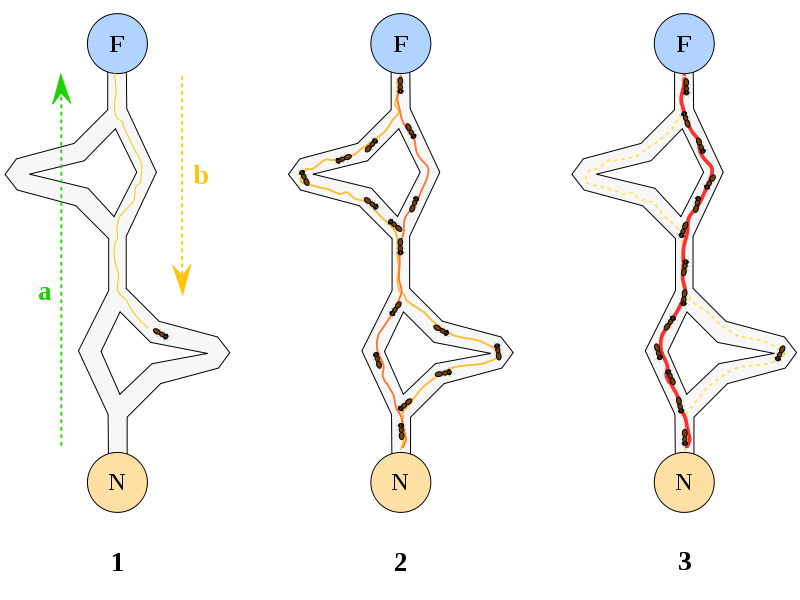
\includegraphics[scale=0.45]{resources/swarm_ant_system.png}
    \caption{Funktionsweise des Ant Systems \cite{Wiki03}}
    \label{fig:swarm}
  \end{figure}

In Grafik \ref{fig:swarm} können wir erkennen, dass die Ameisen nach einer gewissen Zeit die Strecken mit den
höchsten Dufstoffkonzentrationen bevorzugen.

\subsection{Funktionsweise}
Möchte man den Ant System Algorithmus implementieren, müssen bestimmte Parameter berücksichtigt werden. Die
Wahrscheinlichkeiten, dass sich eine Ameise am Knotenpunkt $i$ entscheidet nach $j$ zu krabbeln, kann durch
Formel \ref{eq_ant} berechnet werden \cite{Blu03}. 

\begin{equation}
    \label{eq_ant}
    P_{ij}(t) = \begin{cases}
        \frac{[T_{ij}(t)]^\alpha \cdot [N_{ij}]^\beta}
        {\sum_{j \in {allowed}}^{} [T_{ij}(t)]^\alpha \cdot [N_{ij}]^\beta} & \text{wenn } j \in {allowed} \\
        0 & \, \text{sonst}
        \end{cases}
\end{equation}
\label{eq_ant1}

Der interessanteste Part dieser Formel stellt die Pheromonverteilung [\ref{eq_pheromon}] dar. Sie liefert den Wert
für die Pheromonkonzentration zwischen Knoten $i$ und $j$. Die Pheromonintensität ergibt sich
aus dem vorgängigen Durchlauf $(t-1)$ und den aktuell durchgelaufenen Ameisen $\Delta T_{ij}(t, t+1)$. Sie
unterliegt einem zeitlichen Zerfall, auch Evaporation genannt. Dieser Koeffizient $\rho$  stellt sicher, dass
die Pheromonkonzentration nicht ins Unendliche ansteigen kann; Dementsprechend sollte auch $\rho < 1$ sein.
Die Pheromonwerte jeder Teilstrecke werden nach jedem Durchgang mittels (\ref{eq_pheromon}) neu berechnet.

\begin{equation}
    \label{eq_pheromon}
    T_{ij}(t + 1) = \rho \cdot [T_{ij}(t)] + \Delta T_{ij}(t, t+1)
\end{equation}
\label{eq_pheromon1}

Nebst der Pheromonverteilung existiert noch eine weitere Komponente, nämlich die Sichtbarkeit der einzelnen
Knoten $N_{ij}$. Ameisen richten sich nicht nur nach der Duftintensität der Strecke, sondern bevorzugen
nebenbei auch kürzere Wege. Die Sichtbarkeit kann ganz simpel als $\frac{1}{d_{ij}}$ berechnet werden. Dieser
Ansatz ist Greedy \cite{Wiki04} und könnte auch durch eine ausgefeiltere Heuristik ersetzt werden.

Um nicht die gleichen Knoten mehrfach zu besuchen, wird eine Tabu-Liste eingesetzt. Diese Liste existiert
für jede einzelne Ameise und wird in jedem Durchlauf mit dem aktuell besuchten Knoten erweitert. Folglich
berechnet sich die Liste der erlaubten Knoten aus der Differenz der Liste aller Knoten und der Tabu-Liste,
in (\ref{eq_ant}) als $allowed$ gekennzeichnet.

Durch die Parameter $\alpha \text{ und } \beta$ können die Pheromonverteilung und die Sichtbarkeit
gewichtet werden. Dieses Feintuning kann das Ant System zu einem reinen Greedy-Algorithmus
$(\alpha = 0, \beta = 1)$ oder zu einem Zufallsalgorithmus $(\alpha = 1, \beta = 0)$ verändern.


\subsection{Anwendungsgebiete}
Der Ant System Algorithmus wurde zum Lösen von Kombinationsproblemen entwickelt. Bei diesem Problemtypen
besteht die Schwierigkeit darin, aus mehreren Teillösungen die optimale Kombination zu finden. Die Summe
an möglichen Lösungen übersteigt somit die Kompetenz von traditionellen Pfadsuch-Algorithmen. Wie anfänglich
in Kapitel 1 behandelt, eignen sich Nature-Inspired Algorithmen für diese Aufgaben besonders gut. Da es
sich bei diesen Problemen um heuristische Optimierungsverfahren handelt, kann der Ant System Algorithmus
aber nicht garantieren, jeweils den bestmöglichen Lösungsweg zu finden \cite{Wiki03}.

Mit dieser Art von Kombinationsproblemen beschäftigen sich beispielsweise Logistikunternehmen, um eine
optimale Transportroute zu finden. Weiter kann das Ant System auch zur Konstruktion von Halbleiterplatten
oder bei der Kantendetektion in der Bildverarbeitung eingesetzt werden \cite{Wiki07}.

\subsubsection{Travelling Salesman Problem (TSP)}
Das Problem des Handelsreisenden ist ein bekanntes Beispiel von kombinatorischen Optimierungsproblemen
\cite{Wiki05}. Man versucht eine festgelegte Anzahl Städte zu besuchen, wobei keine Stadt bis auf die
Anfangsstadt mehrfach besucht werden darf. Ziel ist es, einen optimalen Weg zu finden, bei welchem der
Handelsreisende die kleinstmögliche Distanz zurücklegen muss. Das TSP gehört zu den NP-vollständigen
Problemen, daher existiert kein Algorithmus, welcher den optimalen Weg in polynomieller Laufzeit bestimmen
kann \cite{Wiki06}.

\subsection{Erweiterungen}
Das 1991 vorgestellte Ant System wurde mehrfach weiterentwickelt, um sowohl Laufzeit als auch Effizienz zu
verbessern. Die populärsten Weiterentwicklungen werden hier kurz erläutert.

\subsubsection{Elite Ant System (1991)}
Das Elite Ant System unterscheidet sich nur geringfügig vom ursprünglichen Ant System. Es verwendet eine
angepasste Pheromonverteilungsfunktion \cite{MZ14}. Anders als beim Ant System, bei welchem jede Ameise
die gleiche Menge an Pheromonen ausströmt, existieren sogenannte Elite-Ameisen, welche eine grössere Menge
an Duftstoffen ausströmen und so die Kolonie bei der Pfadsuche wesentlicher beeinflussen. Der
nach jeder Iteration kürzeste Pfad wird als Elitepfad angesehen und die darauf wandernden Ameisen sind
folglich die Elite-Ameisen \cite{BHS99}.

\subsubsection{Rank-based Ant System (1997)}
Eine weitere Erweiterung des Ant System stellt das Rank-based Ant System dar. Nach jeder Iteration werden
die Ameisen anhand von ihrem zurückgelegten Pfad der Länge nach sortiert. Ameisen mit den kürzeren Pfaden
tragen anschliessend verhältnismässig mehr zur Pheromonverteilung bei als solche mit längeren. Zusätzlich
werden nur die Anzahl $\omega$ besten Ameisen für die Berechnung verwendet. Dies verringert die Gefähr, dass
eine hohe Pheromonkonzentration durch viele Ameisen auf dem gleichen sub-optimalen Pfad entsteht
\cite{BHS99}.

\subsubsection{Max-Min Ant System (1999)}
Anders als beim Ant System legt nur die beste Ameise ihre Pheromonspur. Desweiteren werden die
Pheromonkonzentrationen pro Teilpfad mit einem Max- und Minimum-Wert versehen. So können keine gänzlich
unattraktiven und auch keine zu stark konzentrierten Pfade entstehen. Wenn die beste Ameise eine Teilstrecke
$ij$ nicht passiert hat, ist der dazukommende Pheromonwert als $\Delta T_{ij}^\text{best} = 0$ definiert
\cite{Dor07}.


\section{Bees Algorithm}
Eine Kolonie Honigbienen schwärmt bei ihrer Suche nach Nektar in einem Radius von über 10km in alle Richtungen
aus. Blumenfelder mit einer grossen Menge an Nektar oder Pollen für die Nachkömmlinge, sollen von einer
grösseren Menge Bienen angeflogen werden als kleinere Felder mit weitaus weniger Nektar oder Pollen. Sogenannte
Erkundungsbienen, welche zur Klasse der Arbeiterbienen gehören, fliegen zufällige Blumenfelder an. Zurück im
Bienenstock evaluieren die Erkundungsbienen die gefundenen Blumenfelder anhand verschiedener Kriterien wie
Nektarmenge oder Distanz zum Bienenstock. Mit einem Wackeltanz kommunizieren die Bienen ihre Ergebnisse mit
der restlichen Kolonie. Aus dem Wackeltanz können die Bienen die Richtung zum Blumenfeld, die zurückzulegende
Distanz und die ungefähre Nektarmenge ableiten \cite{Bro11}.

Diese einzigartige Fertigkeit lässt die Bienenkolonie immer die gerade passende Anzahl an Arbeiterbienen an
Blumenfelder in ihrem Suchradius ausschwärmen.

\subsection{Funktionsweise}

\subsection{Anwendungsgebiete}